\documentclass{report}
\usepackage{quentin}
\definecolor{mycolor}{HTML}{00519d}
\definecolor{darkWhite}{rgb}{0.94,0.94,0.94}
\usepackage{enumitem}
%\usepackage{luacode,numprint,fourier}
\usepackage{hyperref}
\usepackage{pgfplots}
\usepackage{mathtools}
\usepackage{graphicx}
\usepackage{pdfpages}
\usepackage[backend=biber]{biblatex} %backend tells biblatex what you will be using to process the bibliography file
\addbibresource{bib.bib}

\AddToShipoutPicture*{
\begin{tikzpicture}[remember picture, overlay]

\draw[fill=mycolor!50,draw=mycolor!50](current page.north west)rectangle([yshift=-\paperheight/24]current page.north east);
\draw[draw=mycolor!60, line width=1.5mm]([yshift=-\paperheight/24]current page.north west)--([yshift=-\paperheight/24]current page.north east);

\draw[fill=mycolor!50,draw=mycolor!50](current page.south west)rectangle([yshift=\paperheight/24]current page.south east);
\draw[draw=mycolor!60, line width=1.5mm]([yshift=\paperheight/24]current page.south west)--([yshift=\paperheight/24]current page.south east);
\end{tikzpicture}
}


\begin{document}


\titre{
\Huge\textbf{Documentation des cartes de protections}\\[0.2cm]
\large\textbf{Pour le calculateur analogique}\\
\rule{\linewidth}{0.5mm}
\\[2cm]
\LARGE Quentin \textsc{Caldeira}
}


\tableofcontents
\thispagestyle{empty}
\entete
\newpage
\thispagestyle{empty}
\listoffigures
\entete
\listoftables
\entete



\chapter{Contexte}
\thispagestyle{empty}
La carte a pour objectif d'interfacer une face avant avec une carte d'acquisition. Son but est de protéger la carte de potentielles mauvaises manipulations. Étant donné le coût d'une carte d'acquisition, la carte de protection doit protéger la carte d'acquisition. Dans le pire des cas, il est préférable que ce soit la carte de protection qui soit détruite, plutôt que la carte d'acquisition. L'idéal reste qu'aucun des deux éléments ne soit détruit. On souhaite principalement se protéger des courts-circuits et de tensions trop élevées.Une première carte a été réalisée en 1993. Cette carte est fonctionnelle, mais présente quelques défauts qui seront explicités. Cette nouvelle carte a pour objectif de corriger les défauts de l'ancien modèle, de réduire le nombre d'entrées/sorties, et de donner un coup de jeune à la carte.


\chapter{Présentation de l'existant}
\thispagestyle{empty}
Cette partie détaillera les cartes précédemment installées dans le calculateur. La carte dispose de 20 entrées et 12 sorties. Il semblerait qu'elle ait été conçue ainsi afin d'utiliser toutes les broches inférieures du connecteur fond de panier. Le connecteur utilisé est un DIN 41612 de 64 broches. Il s'avère qu'au quotidien, seulement 8 entrées et 2 sorties sont utilisées au maximum. La carte mesure 10 cm de largeur et 22 cm de longueur. C'est une taille standard que toutes les cartes insérées dans les racks doivent respecter. Les connecteurs utilisés sur la face avant sont des connecteurs banane, de couleurs différentes en fonction d'une entrée, d'une sortie ou d'une masse. Il n'y a pas de détrompeur entre les 3 connectiques.

\section{Les cartes d'acquisition}
Les cartes d'acquisition précédemment utilisées étaient des NI PCI 6014 et NI PCI 6024E. Ces cartes sont au format PCI. Les spécifications de cette carte sont synthétisées dans le tableau ci-dessous.

\begin{center}
\begin{table}[h!]
\begin{tabular}{l|l|l|}
\cline{2-3}
                                                                 & Entrée                                 & Sortie                   \\ \hline
\multicolumn{1}{|l|}{Tension d'E/S max en fonctionnement normal} & $\pm 10 V$                             & $\pm 10 V$               \\ \hline
\multicolumn{1}{|l|}{Impédance d'entrée/sortie}                  & 100 G$\Omega$ en parallèle avec 100 pF & 0,1 G$\Omega$            \\ \hline
\multicolumn{1}{|l|}{Protection contre les tensions (On/Off)}    & 25 / 15 V                              & Court-circuit à la masse \\ \hline
\multicolumn{1}{|l|}{Courant de sortie max}                      & -                                      & 5 à 10 mA                \\ \hline
\multicolumn{1}{|l|}{Courant d'entrée max}                       & -                                      & 5 à -10 mA               \\ \hline
\end{tabular}
\caption{Spécifications des cartes PCI 6014 et PCI 6024E}
\end{table}
\end{center}

\section{Alimentation des amplificateurs}
Comme les amplificateurs utilisés sont alimentés en $\pm$15 V, et que les cartes ont une alimentation par défaut de $\pm$24 V, il a fallu adapter cette tension. Des régulateurs de tensions positifs et négatifs ont été utilisés. Un 7815CT a été utilisé pour générer la tension +15 V, et un 7915 pour la tension -15 V. Des capacités de filtrage ont été placés en amont et en aval des alimentations, ainsi que des diodes de protections servant à prévenir des inversions de polarité. La mise en place d'un tel circuit est explicité sur la \bsc{Figure} \ref{fig:alim_exist}. Le choix des capacités se fait souvent en fonction de la documentation du constructeur. De plus, des dissipateurs thermiques ont étés placé afin de limiter la chauffe des régulateurs de tension.

\newpage%%%%%%%%%%%%%%%%%%
\begin{figure}[!h]
\centering
\begin{circuitikz}
\ctikzset{multipoles/thickness=3}
\ctikzset{multipoles/dipchip/width=2}



\draw (0,0) node[dipchip,
num pins=6, hide numbers, no topmark,
external pins width=0](C){7815CT};
\node [right, font=\tiny] at (C.bpin 2) {Vin};
\node [left, font=\tiny] at (C.bpin 5) {Vout};
\draw (C.s)node[above,font=\tiny]{GND} -- ++(0,-1) node[ground]{};

\draw(C.bpin 2)to[empty diode,invert]++(-3,0)node[left]{+24 V};
\draw(C.bpin 2)--++(-.5,0)to[C,l_=22pF]++(0,-2);
\draw(C.bpin 5)--++(.5,0)to[C,l=22pF]++(0,-2)--++(-1.9,0)--++(-1.9,0);
\draw(C.bpin 5)--++(2,0)node[right]{+15 V};

\draw (0,-4) node[dipchip,
num pins=6, hide numbers, no topmark,
external pins width=0](C){7915};
\node [right, font=\tiny] at (C.bpin 2) {Vin};
\node [left, font=\tiny] at (C.bpin 5) {Vout};
\draw (C.s)node[above,font=\tiny]{GND} -- ++(0,-1) node[ground]{};

\draw(C.bpin 2)to[empty diode]++(-3,0)node[left]{-24 V};
\draw(C.bpin 2)--++(-.5,0)to[C,l_=22pF]++(0,-2);
\draw(C.bpin 5)--++(.5,0)to[C,l=22pF]++(0,-2)--++(-1.9,0)--++(-1.9,0);
\draw(C.bpin 5)--++(2,0)node[right]{-15 V};

\end{circuitikz}
\caption{Schéma de principe de protection de l'alimentation sur la carte existante}
\label{fig:alim_exist}
\end{figure}


\section{Protection des entrées}
\subsection{Présentation}

Afin de protéger les entrées, le montage sur la \bsc{Figure} \ref{fig:entree_exist} a été utilisé. Ce montage possède deux diodes Zener en tête-bêche afin d'écrêter la tension à $\pm$10 V. Une résistance de 1 M$\Omega$ est placée en entrée, ainsi qu'en contre-réaction. Une résistance de 1 k$\Omega$ est placée en sortie afin de limiter le courant. Comme la tension de sortie sera de maximum 10 V, le courant devrait être de maximum 10 mA. Le montage est de type \textbf{inverseur}, ce qui veut dire que le gain est d'environ \textbf{-1}. Une entrée à +10 V sera vue comme -10 V par la carte d'acquisition. Ce gain négatif est corrigé par le logiciel qui récupère les signaux (\bsc{MatLAB} en l'occurence). L'amplificateur opérationnel est monté sur un socket DIP-14, afin qu'il soit remplaçable facilement.

\begin{figure}[!h]
\centering
\begin{circuitikz}[european]
\ctikzset{resistors/scale=0.7, capacitors/scale=0.7, diodes/scale=0.7, inductors/scale=0.7}
\draw (0,0) node[op amp,scale=1] (opamp) {};
\draw (opamp.-) --++ (-.5,0)node(b){}--++(0,1)node(a){}to[name=r1,R,l=1M$\Omega$]++(3,0)--++(0,-1.49)node(c){} to (opamp.out);
\draw (a.south)--++(0,1)to[Zener diode]++(1.5,0)to[Zener diode,invert]++(1.5,0)--++(0,-1);
\draw (b.east)to[R,l=1M$\Omega$]++(-2,0)node[left]{Entrée};
\draw (c.west)to[R,l=1k$\Omega$]++(2,0)node[right]{Carte d'acquisition};
\draw (opamp.+)node[ground]{};
\draw (opamp.up) --++ (0,.2) node[above] {15 V};
\draw (opamp.down) --++ (0,-.2) node[below] {-15 V};
\end{circuitikz}
\caption{Schéma de principe de protection des entrées sur la carte existante}
\label{fig:entree_exist}
\end{figure}

\subsection{Mesures}
Pour les entrées, il n'y a pas trop de soucis de protection. En injectant 10 V en entrée, on récupère bien environ -10 V en sortie. Lorsqu'une tension d'alimentation telle que -15 V est injectée, la tension est bien limitée à environ 10 V.

\section{Protection des sorties}
\subsection{Présentation}

Afin de protéger les sorties, le montage sur la \bsc{Figure} \ref{fig:sortie_exist} a été utilisé. Ce montage possède un filtre passe-bas du 1$^{er}$ ordre. L'intérêt d'un tel filtre est discutable, car le signal provient de la carte d'acquisition. Un deuxième filtre passe-bas est placé dans la contre-réaction de l'amplificateur opérationnel. En sortie de ce montage, une résistance de 1 k$\Omega$ a été placée afin de limiter le courant en cas de court-circuits. Cette résistance pose problème car de manière générale, dans un circuit, on cherche à avoir une forte impédance d'entrée et une faible impédance de sortie. On cherche cela afin de faciliter les adaptations d'impédances, c'est-à-dire que la majorité des courants circulant dans un circuit n'ont pas d'impact sur l'autre circuit raccordé. Hors, il a été remarqué qu'avec cette résistance, une chute de tension est observée sur certains procédés.

\begin{figure}[!h]
\centering
\begin{circuitikz}[european]
\ctikzset{resistors/scale=0.7, capacitors/scale=0.7, diodes/scale=0.7, inductors/scale=0.7}
\draw (0,0) node[op amp,scale=1] (opamp) {};
\draw (opamp.-) --++ (-.5,0)node(b){}--++(0,1)node(a){}to[name=r1,R,l=1M$\Omega$]++(3,0)--++(0,-1.49)node(c){} to (opamp.out);
\draw (a.south)--++(0,1)to[C,l=22pF]++(3,0)--++(0,-1);
\draw (b.east)to[R,l=1M$\Omega$]++(-3,0)node[left]{Carte d'acquisition};
\draw (b.west)--++(-0.5,0)--++(0,-0.5)to[C,l=10nF]++(0,-0.5)node[ground]{};
\draw (c.west)to[R,l=1k$\Omega$]++(2,0)node[right]{Sortie};
\draw (opamp.+)node[ground]{};
\draw (opamp.up) --++ (0,.2) node[above] {15 V};
\draw (opamp.down) --++ (0,-.2) node[below] {-15 V};
\end{circuitikz}
\caption{Schéma de principe de protection des sorties sur la carte existante}
\label{fig:sortie_exist}
\end{figure}

\subsection{Mesures}
Pour la sortie, des mesures ont d'abord été faites pour estimer la chute de tension. Sur le procédé de régulation de température par exemple, pour une tension de 10 V fournie par la carte NI, nous ne récupérons que 9 V sur le procédé, soit une chute de 1 V pour 2 mA de consommation. La solution actuelle pour palier à ce problème est de passer par un deuxième amplificateur opérationnel qui a rôle de \textbf{buffer}, c'est-à-dire de faire le lien entre deux étages grâce à sa forte impédance d'entrée et sa faible impédance de sortie. Cependant, cette solution n'est pas viable, car la protection du deuxième amplificateur n'est pas forcément dimensionné pour respecter l'intégrité de la carte.

Lors d'un court-circuit à la masse, le courant est de l'ordre d'une vingtaine de mA, ce qui est tolérable. Cependant, lorsqu'on court-circuite aux alimentations, le courant est de $\pm$ 35 mA, qui est le courant maximal que l'amplificateur peut débiter en court-circuit. Dans ces situations, c'est l'amplificateur qui fait la sécurité et plus le reste du circuit, en fonctionnant en dégradé. Cela peut occasionner une chauffe trop importante et une destruction de l'AOp.

\section{Connecteur fond de panier}
Afin de pouvoir lier les entrées/sorties du PCB à la carte d'acquisition, le PCB dispose d'un connecteur 64 broches qui vient se connecter à une fiche 64 broches placée en fond de rack. Un câble relie ensuite cette fiche à la carte d'acquisition. Les connexions au connecteur 64 broches se faisaient comme sur la \bsc{Figure} \ref{fig:64_old}. On peut voir qu'une ligne sert aux alimentations et une autre sert aux entrées/sorties. 

\begin{figure}[h!]
\begin{center}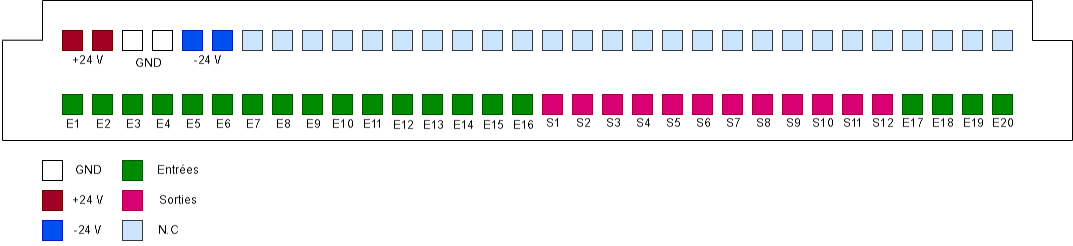
\includegraphics[scale=.4]{IMAGES/fond_de_panierancien.png} 
\end{center}
\caption{Connexions entre le PCB et le connecteur 64 broches fond de panier}
\label{fig:64_old}
\end{figure}

\section{La face avant}


La précédente face avant, c'est-à-dire l'interface entre les utilisateurs et la carte, était comme sur la \bsc{Figure} \ref{fig:face_avant_old}.
Cette face avant dispose de 20 entrées analogiques numérotées en jaune, et 8 sorties analogiques numérotées en rouge. Une fiche de masse est mise à disposition pour pouvoir y connecter des appareils de mesures. La face avant dispose de quatre vis permettant de la fixer au support, et deux vis supplémentaires permettant de fixer la face avant au PCB. Toutes les entrées sorties sont des fiches banane. Ces fiches banane sont ensuite reliées à l'intérieur de la carte par des \textbf{câbles}, soudés aux différents points des entrées/sorties. Cette liaison est montrée dans la \bsc{Figure} \ref{fig:liaison_pcb_old}.
\bigbreak
\begin{minipage}{0.45\textwidth}
\centering
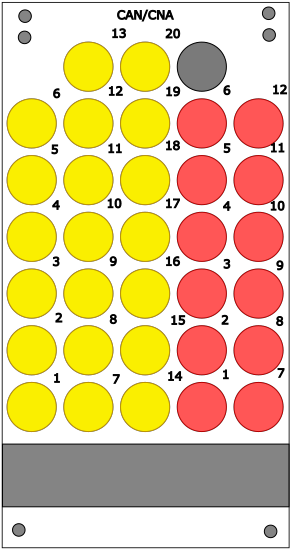
\includegraphics[scale=.6]{IMAGES/face_avant_old.png} 

\captionof{figure}{Face avant de l'ancienne carte}
\label{fig:face_avant_old}
\end{minipage}
\hfill
\begin{minipage}{0.45\textwidth}
\centering
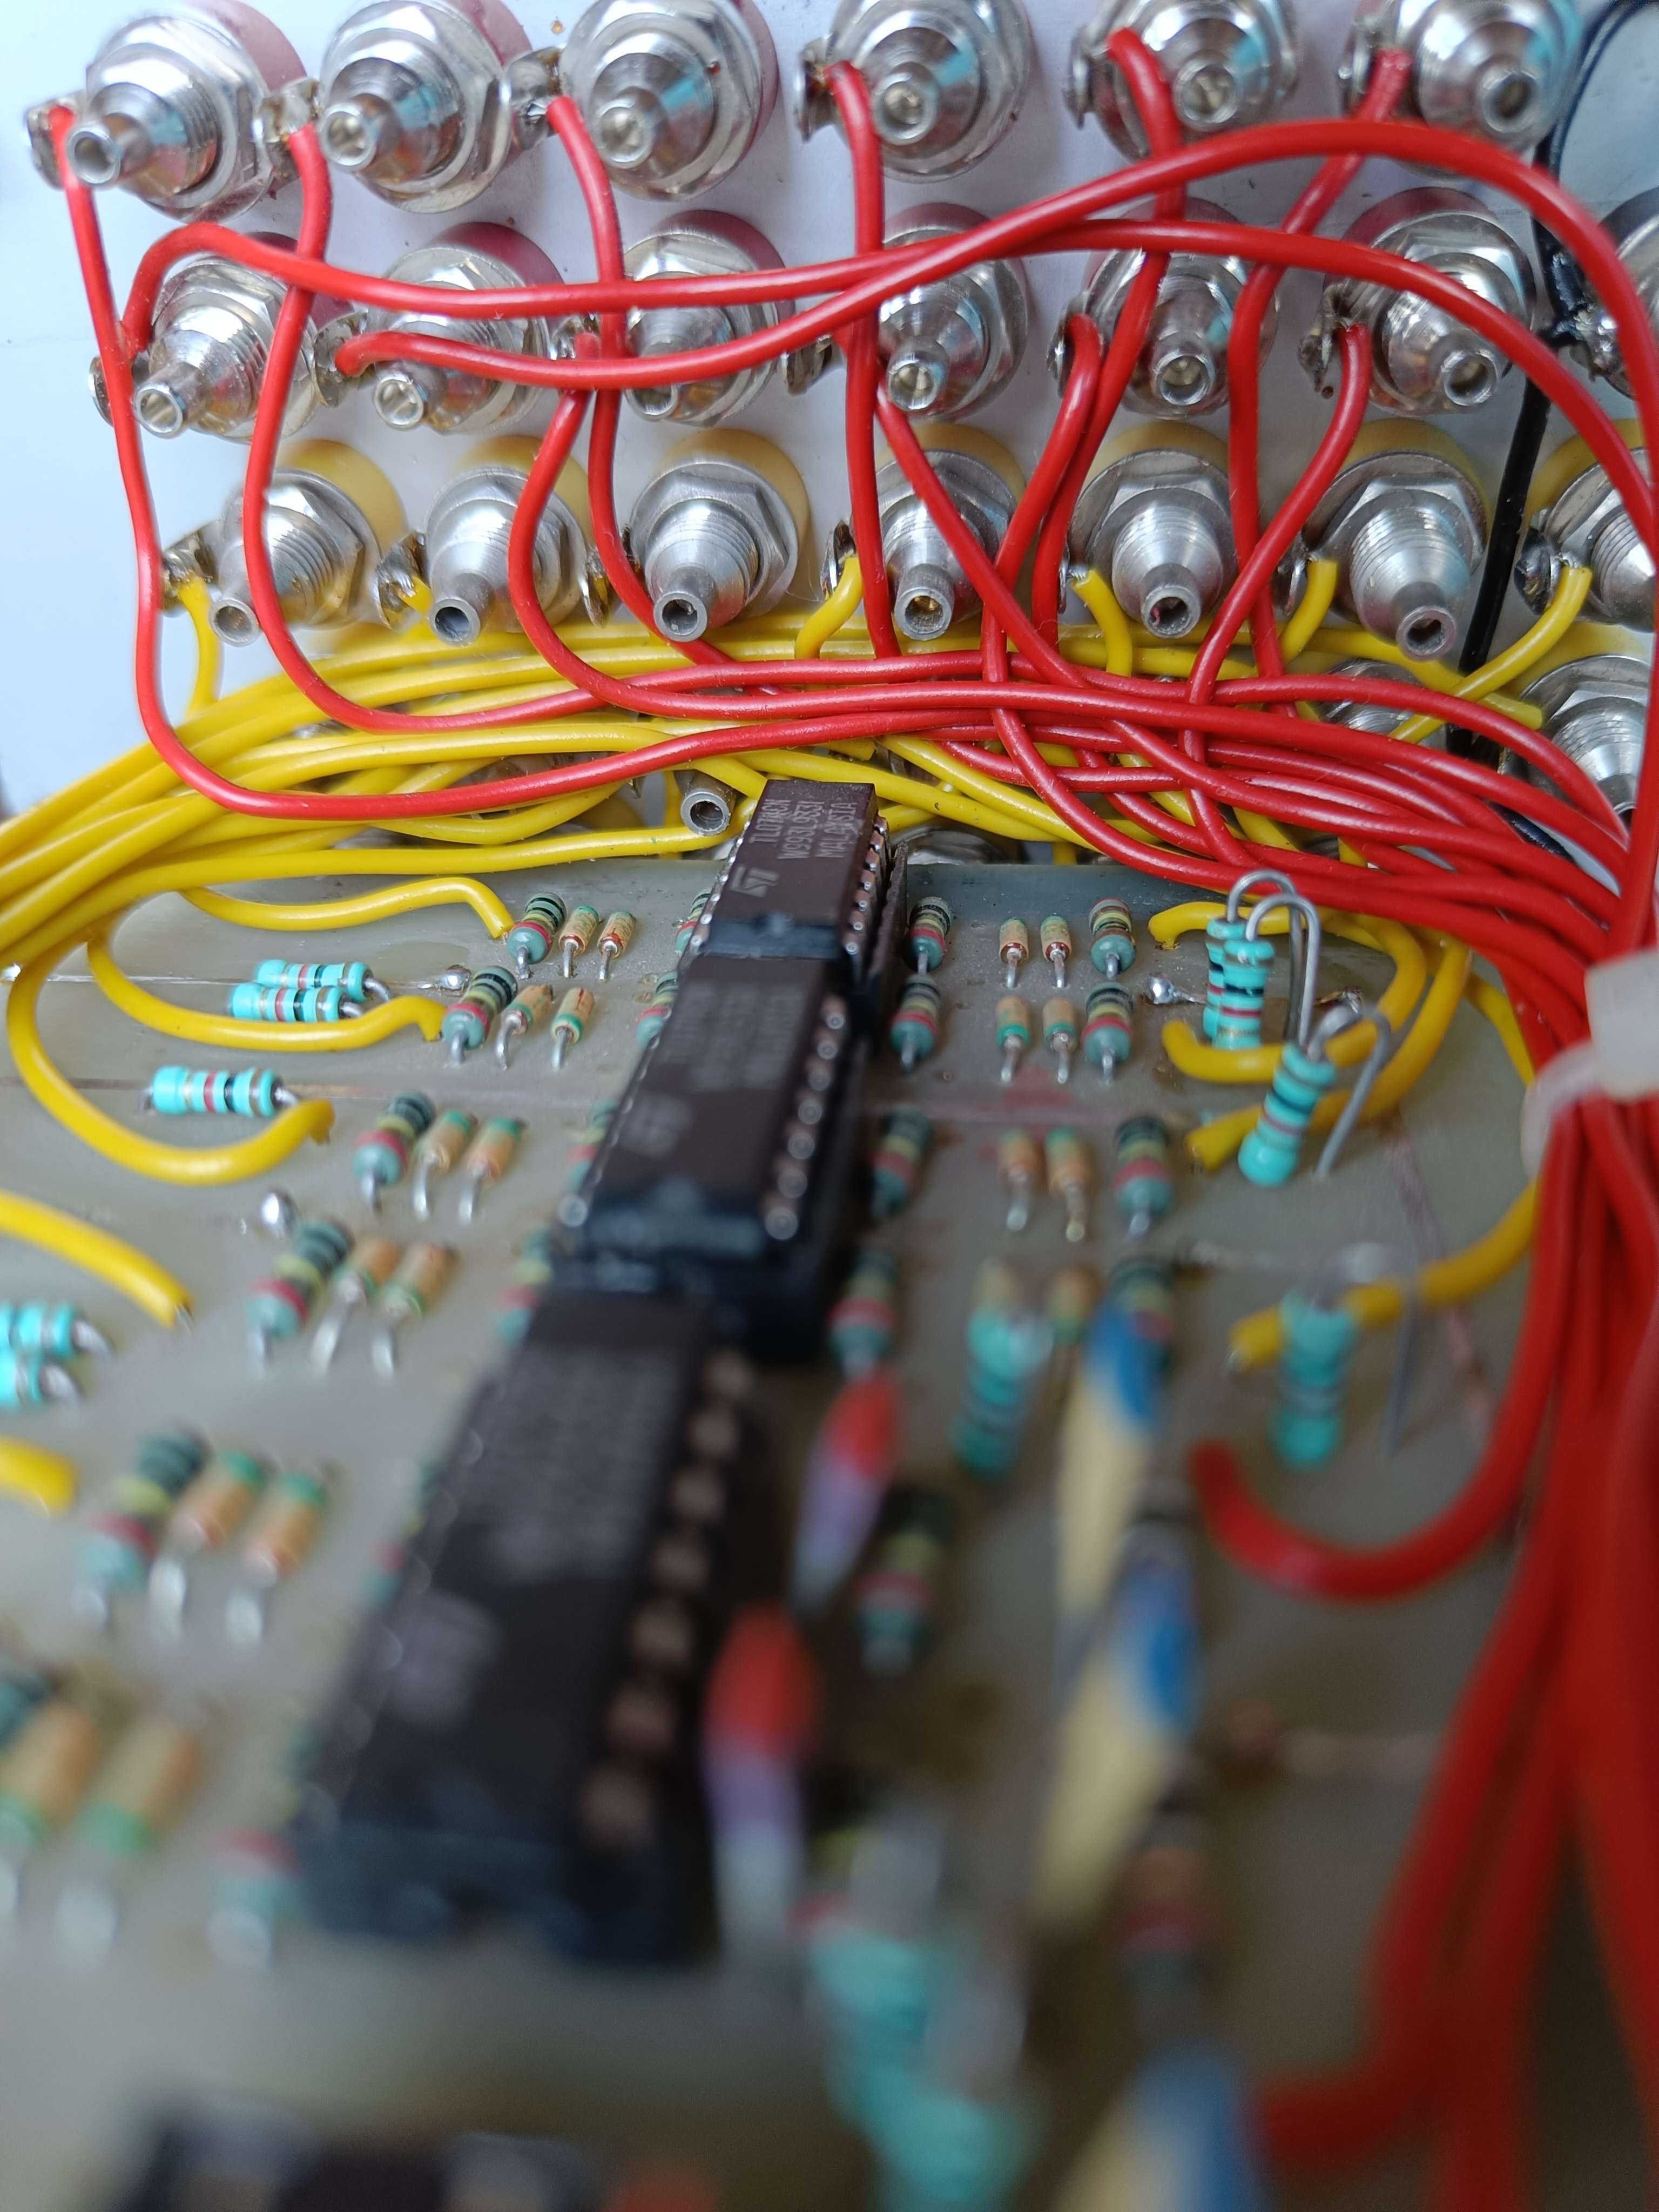
\includegraphics[scale=.0605]{IMAGES/liaison_pcb_old.jpg} 

\captionof{figure}{Connexion des fiches bananes au PCB}
\label{fig:liaison_pcb_old}
\end{minipage}

\chapter{Contraintes de la nouvelle carte}
\thispagestyle{empty}

Maintenant que l'existant est plus claire, il faut dresser un cahier des charges qui permettra de dimensionner les nouveaux éléments de la carte. Il est à noter que le laboratoire a décidé de faire évoluer ses cartes d'acquisitions, abandonnant le format PCI pour le format PCIe. Les nouvelles cartes seront des NI PCIe 6321 et NI PCIe 6323. Il faudra donc dimensionner le circuit pour respecter les contraintes de ces nouvelles cartes.

\section{Etude des nouvelles cartes d'acquisitions}
Les nouvelles cartes étant différentes, il faut prêter attention à leurs spécifications. Ces dernières sont synthétisées dans le tableau ci-dessous.

\begin{table}[!h]
\begin{center}
\begin{tabular}{l|l|l|}
\cline{2-3}
                                                                 & Entrée                                & Sortie       \\ \hline
\multicolumn{1}{|l|}{Tension d'E/S max en fonctionnement normal} & $\pm 11 V$                            & $\pm 10 V$   \\ \hline
\multicolumn{1}{|l|}{Impédance d'entrée/sortie}                  & 10 G$\Omega$ en parallèle avec 100 pF & 0,2 $\Omega$ \\ \hline
\multicolumn{1}{|l|}{Protection contre les tensions (On/Off)}    & $\pm$25 / 15 V                        & $\pm$ 15 V   \\ \hline
\multicolumn{1}{|l|}{Courant de sortie max}                      & -                                     & 5 mA         \\ \hline
\multicolumn{1}{|l|}{Courant d'entrée max}                       & $\pm$ 20 mA pendant une surtension    & 5 mA         \\ \hline
\multicolumn{1}{|l|}{Courant de court-circuit}                   & -                                     & $\pm$ 15 mA  \\ \hline
\end{tabular}
\caption{Spécifications des cartes PCIe 6321 et PCIe 6323}
\end{center}
\end{table}

\section{Ajouts par rapport à l'ancienne version}
\subsection{Réduction du nombre d'E/S}
Il s'avère que la carte précédente a été surdimensionnée à l'époque. En effet, sur les 20 entrées présentes, seulement huit sont utilisées au maximum simultanément. Il en va de même pour les sorties, seulement deux sont utilisées au maximum simultanément. Une réduction du nombre d'entrées/sorties permettra un gain de place sur la carte, mais facilitera aussi l'ajout de nouvelles fonctionnalités. Il est à noté que les nouvelles cartes partagent la même disposition que les anciennes en ce qui concerne les entrées/sorties analogiques. Il n'y aura donc pas de modifications à apporter à ce sujet.

\subsection{PWM}
Le laboratoire à pour volonté de vouloir ajouter deux sorties PWM par carte, afin de pouvoir piloter des procédés. Il faudra veiller à protéger efficacement cette sortie PWM, comme les sorties analogiques, en cas de mauvais branchement.

\subsection{Encodeur}
Le laboratoire souhaite aussi ajouter deux entrées d'encodeur par carte, afin de pouvoir acquérir la position des moteurs sur des procédés. Il faudra veiller à protéger efficacement cette entrée d'encodeur, comme les entrées analogiques, en cas de mauvais branchement.

\section{Cahier des charges}
\subsection{Dimensions}
La carte devra être aux dimensions du rack de laboratoire, c'est à dire 22 cm de longueur pour 10 cm de largeur maximum.

\subsection{Protection des entrées analogiques}
Les entrées seront manipulées par les élèves. Il faut que ces entrées soient :
\begin{itemize}
\item De couleur différente par rapport aux sorties, PWM et encodeurs
\item Munies de prises bananes pour accueillir les câbles mis à disposition dans le laboratoire
\item Au nombre de 8 par carte
\item Protégées de sorte à ce que la tension arrivant à la carte ne dépasse pas $\pm$ 10 V
\item Protégées de sorte à ce que le courant arrivant à la carte ne dépasse pas $\pm$ 20 mA
\item Facilement réparable, c'est-à-dire qu'un composant griller soit facilement remplaçable
\item De gain le plus proche de 1, c'est-à-dire que le signal émis en entrée doit être le même que celui reçu par la carte, dans un fonctionnement normal
\end{itemize}

\subsection{Protection des sorties analogiques}
Les sorties seront manipulées par les élèves. Il faut que ces sorties soient :
\begin{itemize}
\item De couleur différente par rapport aux entrées, PWM et encodeurs
\item Munies de prises bananes pour accueillir les câbles mis à disposition dans le laboratoire
\item Au nombre de 2 par carte
\item Protégées de sorte à ce que la tension arrivant à la carte ne dépasse pas $\pm$ 15 V
\item Protégées de sorte à ce que le courant sortant de la carte ne dépasse pas $\pm$ 5 mA
\item Facilement réparable, c'est-à-dire qu'un composant griller soit facilement remplaçable
\item De gain le plus proche de 1, c'est-à-dire que le signal émis par la carte doit être le même que celui reçu, dans un fonctionnement normal
\item Avoir une impédance de sortie faible pour permettre une meilleure adaptation d'impédance avec les différentes charges du laboratoire
\end{itemize}

\chapter{Etude des nouvelles protections}
\thispagestyle{empty}
\section{Protection des entrées}
\subsection{Veille technologique}
Dans un premier temps, il est intéressant de se renseigner sur différentes méthodes de protection des entrées. On souhaite principalement se protéger d'une tension d'entrée qui sera trop grande. Une solution simple serait de mettre des diodes Zener en tête-bêche, comme l'illustre parfaitement ce site de l'Université du Mans \cite{Rousseau}. On peut, en choisissant la tension de claquage de la diode, écrêté la tension positive et négative. Cette solution à tout de même une limite. Une résistance est placée en amont pour limiter le courant circulant dans les diodes. Si ce courant devient trop fort, la puissance que la diode devra dissiper deviendra trop élevée et elle sera détruite. Il faut donc correctement dimensionner les diodes et la résistance, en fonction de la tension maximale qu'on risque d'avoir en entrée.

Une autre solution, en utilisant aussi des composants passifs, est de faire comme un pont de résistance et de condensateurs. Cette solution est démontrée dans cet article \cite{FilipovaPetrakieva2020}. Cette solution permet de protéger le circuit contre des surtensions. Même si c'est intéressant de pouvoir s'en protéger, ce circuit sert principalement à protéger des surtensions momentanées et non continue. De ce fait, il ne semble pas adapter à l'application.

Il a aussi été envisagée d'utiliser un \verb+LT4363+ \cite{LT4363AD}, qui est un circuit intégré de Analog Devices permettant de couper le circuit en cas de surtensions, et dispose d'une limitation de courant. Ce composant aurait pu être utilisé mais il est bien trop onéreux pour l'application. Étant donné qu'environ vingt cartes seront fabriquées, mettre un composant à plus d'une dizaine d'euros par entrée analogique n'était pas envisageable, et sûrement surdimensionné pour l'application.

Si on regarde du côté des protections mises sur les microcontroleurs, ce qui peut s'apparenter à une carte d'acquisition avec des niveaux de tension moindre, les solutions semblent toujours être les mêmes. Le site de Digikey \cite{digikey} montre de nombreuses solutions utilisées au quotidien. La première est une simple résistance qui permet de limiter le courant en entrée. Il faut que cette résistance reste négligeable par rapport à l'impédance d'entrée de la carte, qui est de l'ordre du Gigaohm. Une autre solution est d'utiliser des diodes de \textbf{clamping}, qui permettent d'écrêter la tension avant d'aller à la carte, comme précédemment.

Comme dans l'ancienne carte, des amplificateurs opérationnels peuvent être utilisés pour faire un \textbf{buffer}, permettant une bonne adaptation d'impédance et une sorte de \textbf{fusible} artificiel, qui pourrait séparer les deux parties du circuit s'il est détruit. Le séparation n'est pas sûre à 100$\%$, car on ne sait pas comment le composant se comportera en état dégradé, et qu'elles sont les jonctions qui seront crées. Mais, de manière générale, on peut espérer une isolation entre les deux parties.

\subsection{Solution retenue}
Afin de protéger les entrées, le montage sur la \bsc{Figure} \ref{fig:entree_new} a été utilisé. Ce montage possède deux diodes Zener en tête-bêche afin d'écrêter la tension à $\pm$10 V. La saturation de l'amplificateur ne suffira pas à écrêter, car elle dépasse $\pm$10 V. Une résistance de 12 k$\Omega$ est placée en entrée afin de limiter le courant circulant dans les diodes. Un condensateur de 1 nF est placé pour faire un filtre passe-bas. Ce condensateur n'est pas obligatoire et sera retiré pour le moment. Le filtre n'a pas pour volonté d'agir comme un \textbf{filtre anti-repliement}, une carte est déjà prévue à cet effet. Ce filtre a été placé pour nettoyer le signal d'entrée. Une résistance de 150 k$\Omega$ est placée en sortie afin de limiter le courant. Comme la tension de sortie sera de maximum 10 V, le courant devrait être de maximum 10 mA. Il n'y aura donc pas d'inversion de tension à corriger. L'amplificateur opérationnel est monté sur un socket DIP-14, afin qu'il soit remplaçable facilement. Il n'y a pas vraiment de critères de choix pour l'amplificateur. Etant donné que nous sommes sur un montage de type buffer, avec une application plutôt basse fréquence, n'importe lequel ferait l'affaire. Des TL064CN ont donc étés utilisés, afin d'harmoniser les stocks d'amplificateurs avec les cartes de filtres anti-repliement.

\newpage

\begin{figure}[!h]
\centering
\begin{circuitikz}[european]
\shorthandon{;:!?}
\ctikzset{resistors/scale=0.7, capacitors/scale=0.7, diodes/scale=0.7, inductors/scale=0.7}
\draw (0,0) node[op amp,scale=1] (opamp) {};
\draw (opamp.-) --++ (-.5,0)node(b){}--++(0,1)node(a){}--++(3,0)--++(0,-1.49)node(c){} to (opamp.out);
%\draw (a.south)--++(0,1)to[Zener diode]++(1.5,0)to[Zener diode,invert]++(1.5,0)--++(0,-1);
\draw (opamp.+)--++(-2,0)node(zener){}--++(-2,0)node(capa){}to[R,l=12 k$\Omega$]++(-2,0)node[left]{Entrée};
%\draw (b.east)to[R,l=12 k$\Omega$]++(-4,0)node[left]{Entrée};
\draw(capa.east)to[C,l=1 nF]++(0,-2)node[ground]{};
\draw(zener.east)to[Zener diode,l=10 V]++(0,-1)to[Zener diode,invert, l= 10 V]++(0,-1)node[ground]{};

\draw (c.west)to[R,l=150 k$\Omega$]++(2,0)node[right]{Carte d'acquisition};
\draw (opamp.up) --++ (0,.2) node[above] {15 V};
\draw (opamp.down) --++ (0,-.2) node[below] {-15 V};
\end{circuitikz}
\shorthandoff{;:!?}
\caption{Schéma de principe de protection des entrées sur la nouvelle carte}
\label{fig:entree_new}
\end{figure}



\section{Protection des sorties}
\subsection{Veille technologique}
Dans un premier temps, il faut se renseigner sur les méthodes existantes permettant de protéger une sortie. On cherche principalement une protection afin d'empêcher les élèves de détruire la carte en faisant des courts-circuits. Une première solution simple serait d'utiliser des détrompeurs, pour que l'élève ne puisse connecter le câble qu'aux éléments souhaités. Cependant, cette solution n'est pas envisageable car le laboratoire souhaite conserver les fiches bananes pour les manipulations des élèves.
Il est à noter que le calculateur dispose déjà d'un circuit de détection des courts-circuits, pour le bloc d'alimentation uniquement, qui émet un signal sonore et/ou lumineux. Il n'arrête cependant pas le système. Pour rappel le problème actuel est que la résistance utilisée crée une chute de potentiel, par problème d'adaptation d'impédance \cite{Gabriel2012}. Une autre solution pourrait être de trouver une valeur de résistance permettant de limiter le courant à la valeur souhaitée tout en minimisant la chute de tension. Cette solution est envisageable mais difficile à mettre en œuvre car chaque procédé à sa propre impédance d'entrée. Comme on cherche à faire une carte indépendante du procédé, c'est plus compliqué.
Une autre solution est de limiter le courant que peut sortir l'amplificateur opérationnel par ses alimentations. En limitant le courant entrant par les alimentations, on pourra limiter le courant sortant en court-circuit et donc la chauffe du composant. Ce type de montage est montrer sur la note d'application de Texas Instruments \cite{appnoteti}.
En tout cas, il est préférable de continuer à utiliser des amplificateurs opérationnel entre la sortie de la carte d'acquisition et les procédés, comme buffer.

\subsection{Solution retenue}
Afin de protéger les sorties, le montage sur la \bsc{Figure} \ref{fig:sorties_new} a été utilisé. Afin de contrer le problème de la chute de tension liée à une impédance de sortie trop forte du montage, l'idée a été de brider l'amplificateur sur les alimentations. Comme il est souhaitable que le courant en cas de court-circuit soit le plus petit possible, si on limite le courant sur les alimentations, le courant sera limité en court-circuit. Cette limite doit être calculée pour que le circuit puisse tout de même débiter assez de courant pour les procédés. Une résistance de 2 k$\Omega$ est placée en sortie de l'AOp, en amont de la contre-réaction, afin d'aider à limiter le courant. L'AOp est en montage \textbf{non-inverseur}, ce qui veut dire que le gain est d'environ \textbf{1}. Pour chacune des alimentations, il y a d'abord une résistance de 2 k$\Omega$ qui permet de limiter le courant entrant dans l'amplificateur, une capacité de 10 nF en parallèle afin de filtrer l'alimentation, et une diode Zener de 15 V pour aider à contrer les chutes de tensions. En effet, comme le courant absorber est parfois important, la résistance crée une chute de tension trop importante qui va faire saturer l'amplificateur trop vite, donc une diode Zener a été placée en parallèle pour aider à maintenir 15 V dans ces cas-là. Une capacité de 0.1 $\mu$F a été placée entre l'amplificateur et la masse, conformément à la note d'application de Texas Instrument dont est grandement inspiré ce montage. Cette note sera disponible en Annexe. L'amplificateur sera une fois de plus monté sur un socket DIP-14 afin de pouvoir le remplacer facilement. L'amplificateur sera le même que pour la partie entrée, un TL064CN. Il faudra veiller à surdimensionner les résistances en termes de dissipations de puissance, car comme elles brident l'alimentation, elles dissipent beaucoup en chaleur.

\newpage%%%%%%%%
\begin{figure}[!h]
\centering
\begin{circuitikz}[european]
\shorthandon{;:!?}
\ctikzset{resistors/scale=0.7, capacitors/scale=0.7, diodes/scale=0.7, inductors/scale=0.7}
\draw (0,0) node[op amp,scale=1] (opamp) {};
%\draw (opamp.-) --++ (-.5,0)node(b){}--++(0,1)node(a){}--++(5,0)--++(0,-1.49)node(c){}to [R,l=2 k$\Omega$]++(-2,0) to (opamp.out);%%CR-

\draw (opamp.-) --++ (-.5,0)node(b){}--++(0,1)node(a){}to[crossing]++(3.215,0)--++(1.785,0)--++(0,-1.49)node(c){}to [R,l=1 k$\Omega$]++(-2,0) to (opamp.out);%%CR-
\draw (opamp.+)--++(-2,0)node[left]{Carte d'acquisition};


\draw (c.west)--++(1,0)node[right]{Sortie};

%\draw (opamp.up) --++ (0,.2) node[above] {15 V};
\draw (opamp.up) --++ (0,2) node(anch+){};
\draw(anch+.center)to[C,l=0.1 uF]++(2,0)node[ground]{};
\draw(anch+.center)--++(0,1)node(bul){$\bullet$}--++(-2,0)to[Zener diode, l=15 V, invert]++(0,2)--++(2,0)to[R,l=2 k$\Omega$]++(0,-2)--++(2,0)to[C,l_=10 nF]++(0,2)--++(-2,0)--++(0,.2)node[above]{15 V};
\draw (opamp.down) --++ (0,-1) node(anch-){};
\draw(anch-.center)to[C,l=0.1 uF]++(-2,0)node[ground]{};
\draw(anch-.center)--++(0,-1)node(bul){$\bullet$}--++(-2,0)to[Zener diode, l_=15 V]++(0,-2)--++(2,0)to[R,l_=2 k$\Omega$]++(0,2)--++(2,0)to[C,l=10 nF]++(0,-2)--++(-2,0)--++(0,-.2)node[below]{-15 V};
\end{circuitikz}
\shorthandoff{;:!?}
\caption{Schéma de principe de protection des sorties sur la nouvelle carte}
\label{fig:sorties_new}
\end{figure}


\section{Alimentation du circuit}
Pour alimenter le montage, l'alimentation principale sera celle des racks, c'est-à-dire $\pm$24\~V. Les amplificateurs seront eux alimentés en $\pm$15\~V, à l'aide de deux régulateurs de tensions : le 7815CV et le 7915CV. Le montage sera équivalent à celui de la précédente carte, comme le montre la \bsc{Figure} \ref{fig:alim_new}. Les diodes sont des 1N4001.

\begin{figure}[!h]
\centering
\shorthandon{;:!?}
\begin{circuitikz}
\ctikzset{multipoles/thickness=3}
\ctikzset{multipoles/dipchip/width=2}



\draw (0,0) node[dipchip,
num pins=6, hide numbers, no topmark,
external pins width=0](C){7815CV};
\node [right, font=\tiny] at (C.bpin 2) {Vin};
\node [left, font=\tiny] at (C.bpin 5) {Vout};
\draw (C.s)node[above,font=\tiny]{GND} -- ++(0,-1) node[ground]{};

\draw(C.bpin 2)to[empty diode,invert]++(-3,0)node[left]{+24 V};
\draw(C.bpin 2)--++(-.5,0)to[C]++(0,-2);
\draw(C.bpin 5)--++(.5,0)to[C]++(0,-2)--++(-1.9,0)--++(-1.9,0);
\draw(C.bpin 5)--++(2,0)node[right]{+15 V};

\draw (0,-4) node[dipchip,
num pins=6, hide numbers, no topmark,
external pins width=0](C){7915CV};
\node [right, font=\tiny] at (C.bpin 2) {Vin};
\node [left, font=\tiny] at (C.bpin 5) {Vout};
\draw (C.s)node[above,font=\tiny]{GND} -- ++(0,-1) node[ground]{};

\draw(C.bpin 2)to[empty diode]++(-3,0)node[left]{-24 V};
\draw(C.bpin 2)--++(-.5,0)to[C]++(0,-2);
\draw(C.bpin 5)--++(.5,0)to[C]++(0,-2)--++(-1.9,0)--++(-1.9,0);
\draw(C.bpin 5)--++(2,0)node[right]{-15 V};

\end{circuitikz}
\shorthandoff{;:!?}
\caption{Schéma de principe de protection de l'alimentation sur la nouvelle carte}
\label{fig:alim_new}
\end{figure}

\chapter{Intégration des protections dans le calculateur}
\thispagestyle{empty}
\section{Connecteur fond de panier}
Pour les entrées/sorties analogiques, les anciennes et nouvelles cartes d'acquisition n'ont pas changé de disposition des pins. De ce fait, la disposition faite sur la précédente carte de protection pourra être conservée sans avoir à refaire le câble liant le fond de panier à la carte d'acquisition. Les branchements au connecteur fond de panier se feront tel que sur la \bsc{Figure} \ref{fig:64_new}. 

\begin{figure}[h!]
\begin{center}
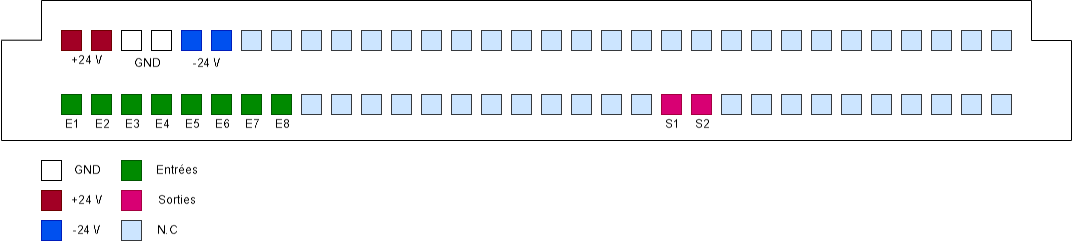
\includegraphics[scale=.4]{IMAGES/fond_de_panier_nouveau.png} 
\end{center}
\caption{Connexions entre le PCB et le connecteur 64 broches fond de panier}
\label{fig:64_new}
\end{figure}

Il est important de ramener les pins non-connectés à la masse, car par défaut la carte fonctionne en mode différentiel. Elle fait donc la différence entre les pins A0 et A8, A1 et A9, etc... Les pattes A8, A9, 10, [...], A15 sont sur les pins non connectés. Le potentiel est donc flottant et la mesure différentielle n'est pas bonne. Il faut donc soit connecté ces pins à la masse, soit faire fonctionner la carte d'acquisition en \textbf{single-ended}, ou encore les deux solutions en même temps. Pour notre part, les pins seront connectés à la masse.

\section{La face avant}
Pour concevoir la nouvelle face avant, on utilise des fiches bananes avec des couleurs différentes en fonction d'une entrée, d'une sortie ou d'une masse. Etant donné que le nombre d'entrées/sorties est moindre, il est intéressant de prendre plus de place sur la face avant afin de mettre des indications visibles et lisibles pour les étudiants. Par ailleurs, sur une face avant, nous pouvons disposer au maximum 8 fiches en longueur et 5 fiches en largeur. Nous n'utiliserons que 4 fiches maximum en largeur, pour que la fixation du PCB à la face avant se fasse de manière plus simple. En temps normal, il faut impérativement que le PCB passe entre deux fiches de la face avant, ce qui est contraignant. Ces quatre idées, visibles sur la \bsc{Figure} \ref{fig:design_face_avant} ont étés proposées aux utilisateurs des calculateurs analogiques.
\newpage
\begin{figure}[!h]
\begin{center}
\includegraphics[width=0.6\textwidth]{IMAGES/design sans dot.png} 
\caption{Différentes idées de face avant}
\label{fig:design_face_avant}
\end{center}
\end{figure}

La face avant qui a été retenue est la deuxième, avec un texte plutôt centré au milieu. Le fichier pour la gravure à été mis à disposition dans le répertoire \verb+ Gravure/face_avant_v1.svg+. Il y a aussi un fichier guide, où les côtes du gabarit présentant 8x5 connecteurs ont étés reportées. Ce fichier peut être utile pour concevoir de nouvelles faces avant. Les paramètres utilisés pour la gravure ont étés :
\begin{itemize}
\item Résolution : 600 dpi
\item Vitesse : 30$\%$
\item Puissance : 50$\%$
\end{itemize}

La gravure a été effectuée sur le côté non protégé des plaques d'aluminium. Il faut bien veiller à placer son dessin en haut à gauche de la feuille sur Inkscape, pour effectuer la gravure. En effet, il y a une équerre dans les graveuses qui permet de positionner la plaque d'aluminium.

\chapter{Design du PCB}
\thispagestyle{empty}
\section{Design}
Pour faire le PCB, le logiciel KiCAD à été utilisé. Le PCB à ensuite été fabriqué par JLCPCB. Les fichiers de conceptions, la liste des composants, ainsi que des copies \verb+pdf+ et \verb+png+ sont disponibles dans le répertoire \verb+PCB+. Un emplacement à été laisser libre pour les condensateurs de filtrage sur le circuit de protection des entrées. De ce fait, une capacité pourra être rajoutée a besoin. Un emplacement pour une résistance additionnelle a été placée en parallèle des résistance de protection des sorties, afin de faire varier sa valeur au besoin. La résistance actuelle à été dimensionnée pour les procédés actuellement utilisés. Si jamais une chute de tension est observé sur de nouveaux procédés, il faudra faire chuter la valeur de cette résistance. Il faut tout de même veiller à ce que les mesures en court-circuit avec cette résistance soit dans une gamme de valeurs non destructive pour la carte, c'est-à-dire inférieur à 35 mA. Des vias ont étés ajoutés pour venir y souder les fils qui relieront la carte à la face avant. Les deux faces sont utilisés, notamment à cause de l'alimentation de la carte qui bloque l'accès à certaines entrées. Un plan de masse à été fait sur la face du dessous pour faciliter le routage.

\section{Problèmes rencontrés}

Un problème rencontré lorsqu'on passe commande auprès de JLCPCB avec un PCB fait sur KiCAD est qu'après lui avoir donner le fichier de placement des composants, les composants sont mal placés sur le PCB. Cela est dû à un problème de normes entre KiCAD et JLCPCB sur certaines empreintes. Une première solution est d'utiliser le logiciel EasyEDA qui fonctionne de paire avec JLCPCB. Une autre solution, qui a été utilisée ici, est un plugin Python du nom de JLC2KiCad. Ce plugin permet de générer des empreintes, symboles et modèles 3D à partir du numéro de référence JLCPCB. Une fiche explicative est disponible dans le répertoire \verb+Tuto+. Avec cette méthode, toutes les empreintes correspondront parfaitement aux composant souhaités.\\

La carte n'a pas été fabriquée aux bonnes dimensions (20 cm par 10 cm au lieu de 22 cm par 10 cm). De ce fait, des extensions plastiques faites à l'imprimante 3d ont été crées afin que la carte rentre parfaitement dans les racks. Les fichiers de conception 3d sont disponibles sur GitHub. La pièce à été conçue sur FreeCAD, un logiciel  open-source.\\

Le dernier soucis rencontré est l'implémentation des vias sur la carte. Des vias ont étés placés pour venir y souder des fils reliant la face avant à la carte. Le problème est que le fabricant ne met pas de pastille de cuivre autour si on met un via sur KiCAD. Les câbles ont donc étés soudés à l'intérieur du via, mais l'opération  est plus compliquée. La connexion se fait tout de même sans problèmes.

\chapter{Caractérisation de la carte}
\thispagestyle{empty}
Les cartes ont étés caractérisées en fréquence et en phase, et les courants en court-circuits ont étés relevés.
\section{Caractérisation des entrées}
Pour caractériser les entrées, un signal sinusoïdal d'amplitude $\pm$5 V à été injecté, et la sortie mesurée à l'oscilloscope.  La réponse en amplitude est visible \bsc{Figure} \ref{fig:ampin} et celle en phase \bsc{Figure} \ref{fig:phiin}.

\begin{figure}[h!]
\begin{center}
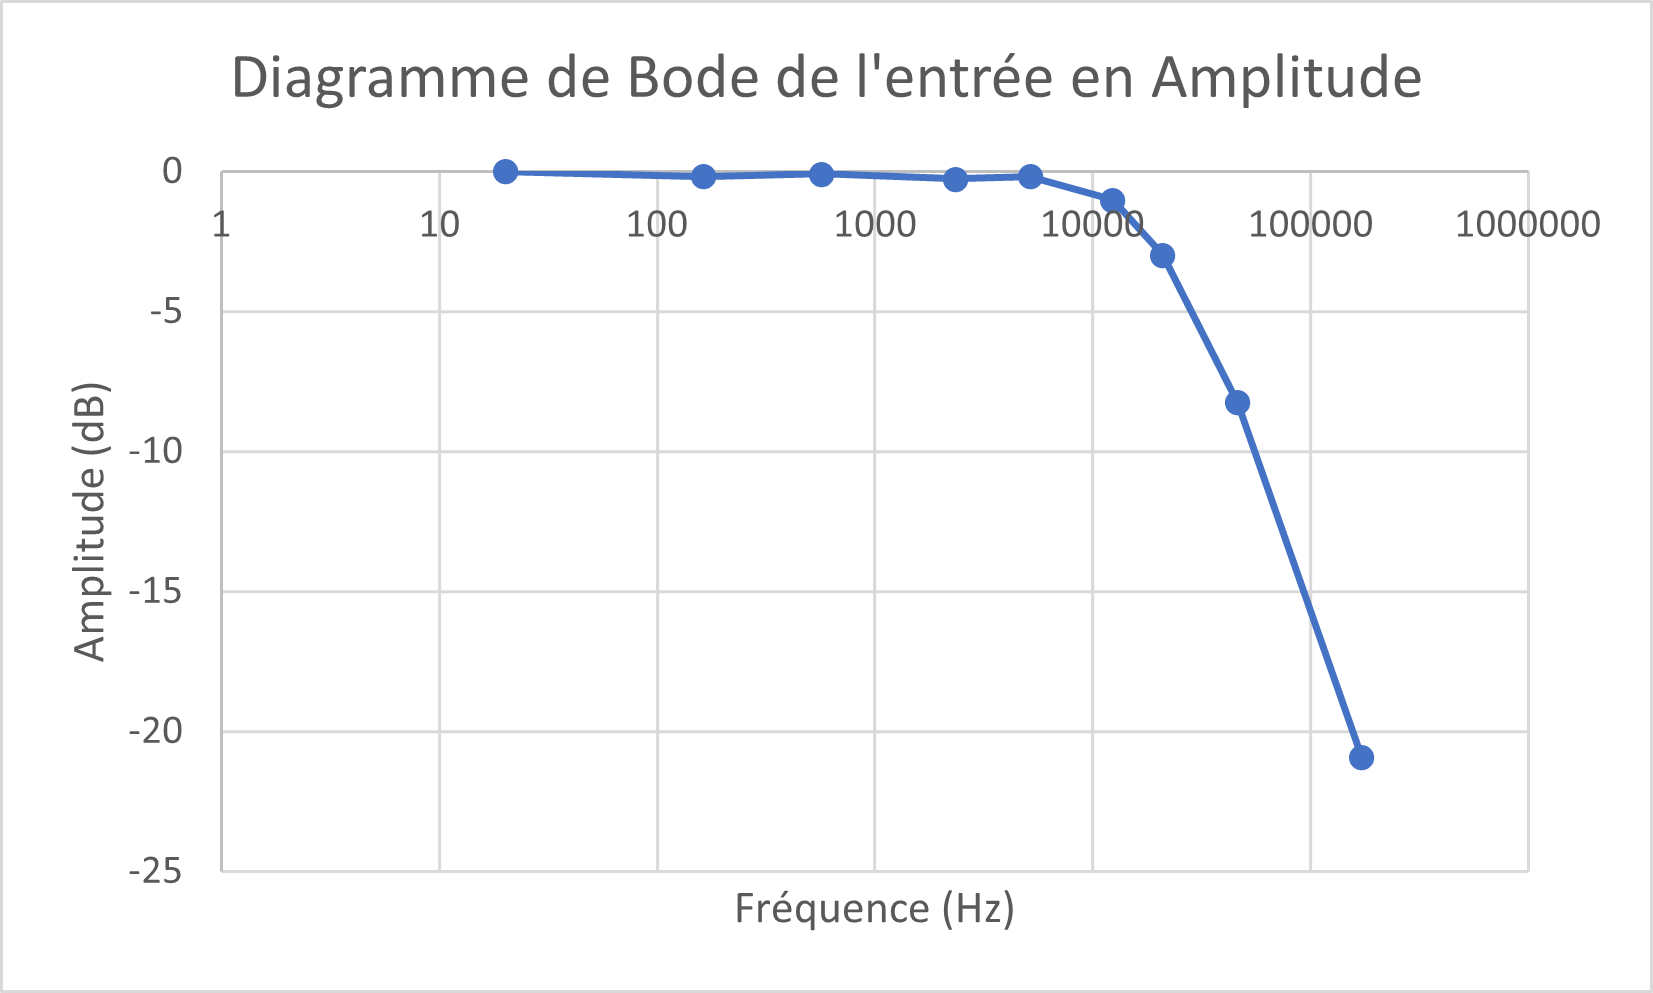
\includegraphics[scale=0.7]{IMAGES/amp_in.png} 
\end{center}
\caption{Diagramme de Bode en amplitude des entrées}
\label{fig:ampin}
\end{figure}

\begin{figure}[h!]
\begin{center}
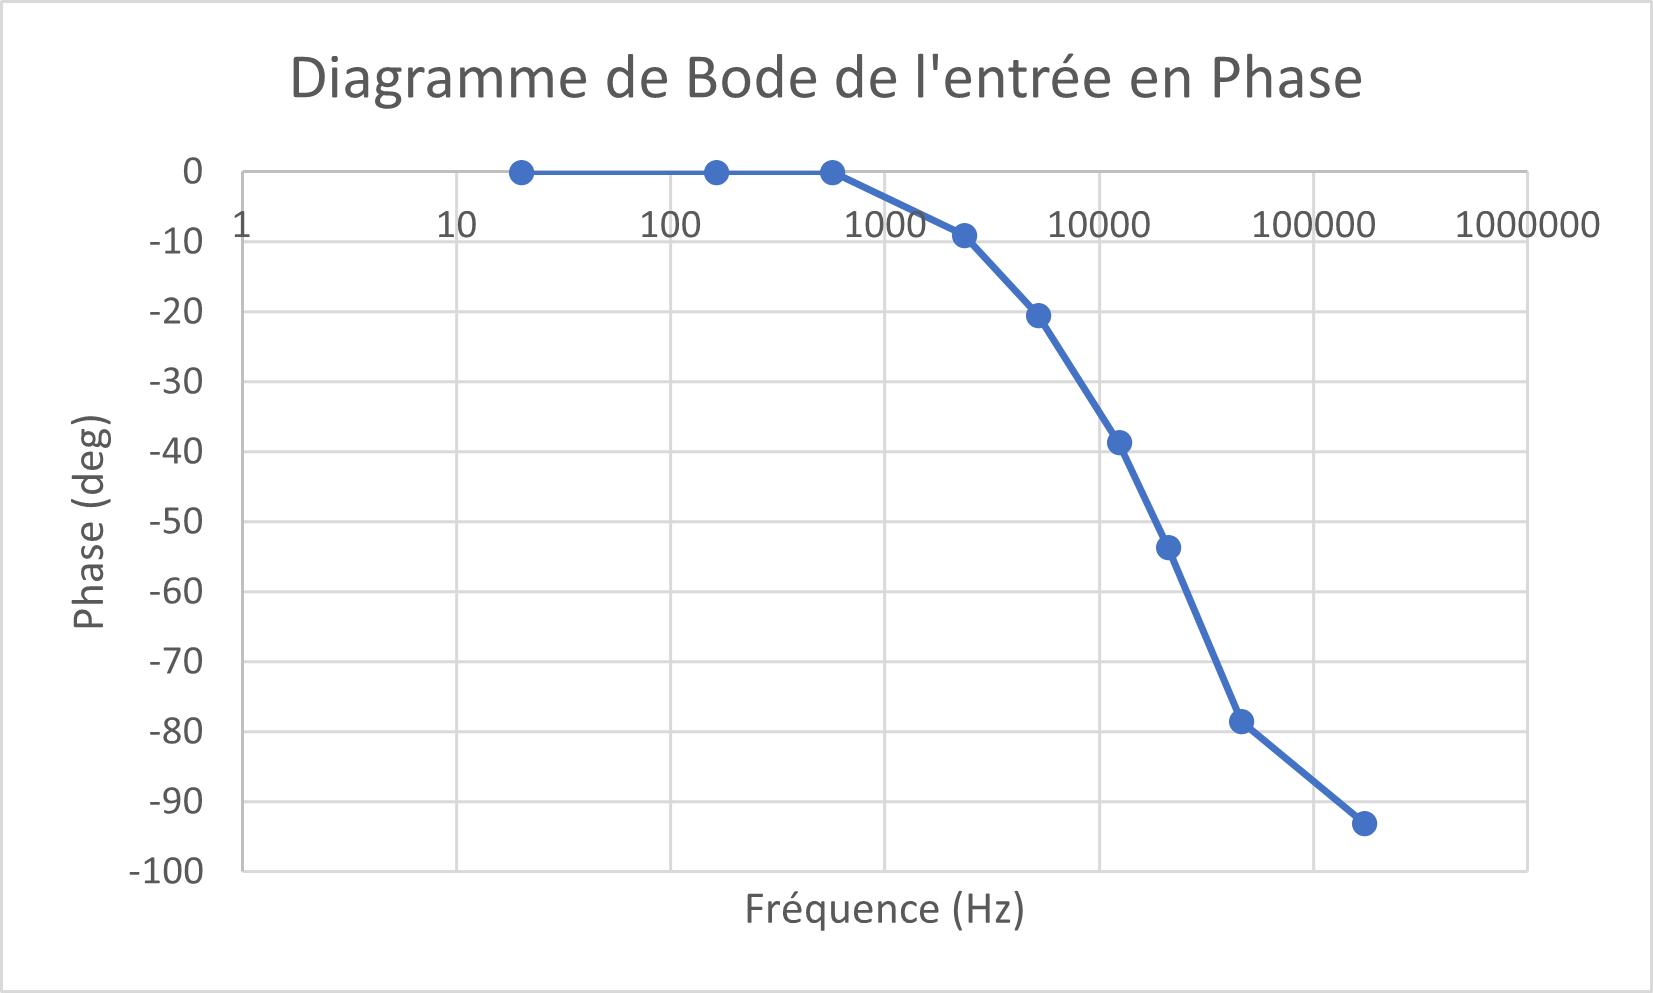
\includegraphics[scale=0.7]{IMAGES/phi_in.png} 
\end{center}
\caption{Diagramme de Bode en phase des entrées}
\label{fig:phiin}
\end{figure}


\section{Caractérisation des sorties}
Pour caractériser les sorties, un signal sinusoïdal d'amplitude $\pm$5 V à été injecté, et la sortie mesurée à l'oscilloscope.  La réponse en amplitude est visible \bsc{Figure} \ref{fig:ampout} et celle en phase \bsc{Figure} \ref{fig:phiout}.

\begin{figure}[h!]
\begin{center}
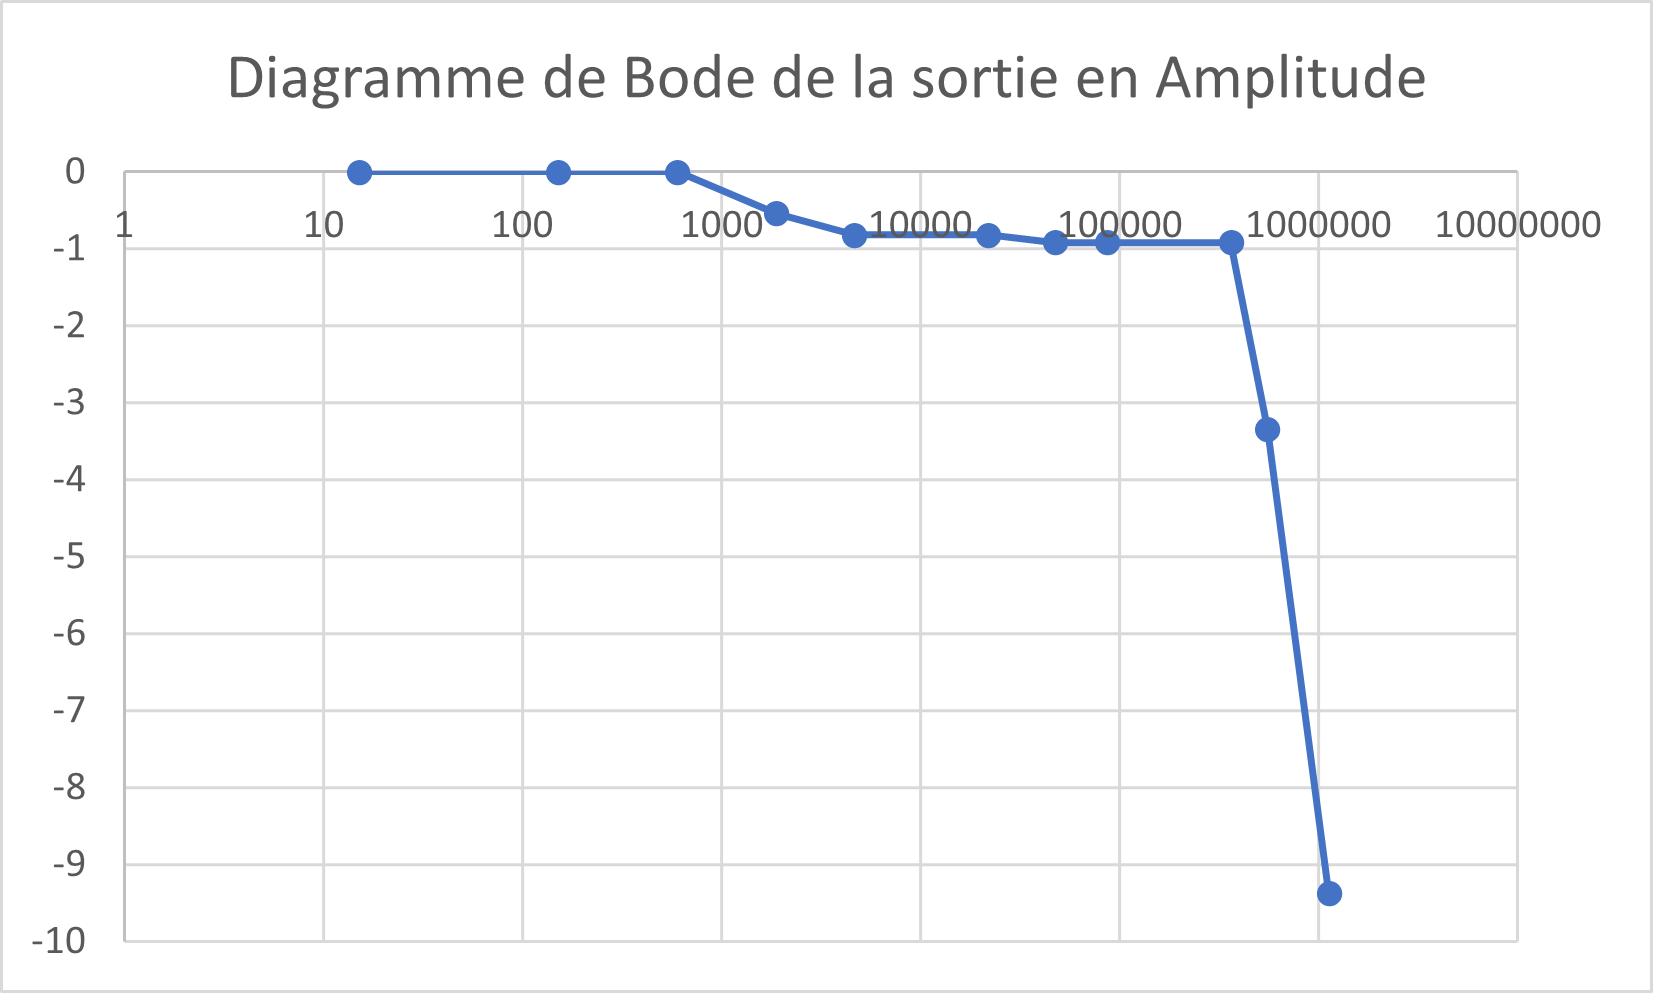
\includegraphics[scale=0.7]{IMAGES/amp_out.png} 
\end{center}
\caption{Diagramme de Bode en amplitude des sorties}
\label{fig:ampout}
\end{figure}

\begin{figure}[h!]
\begin{center}
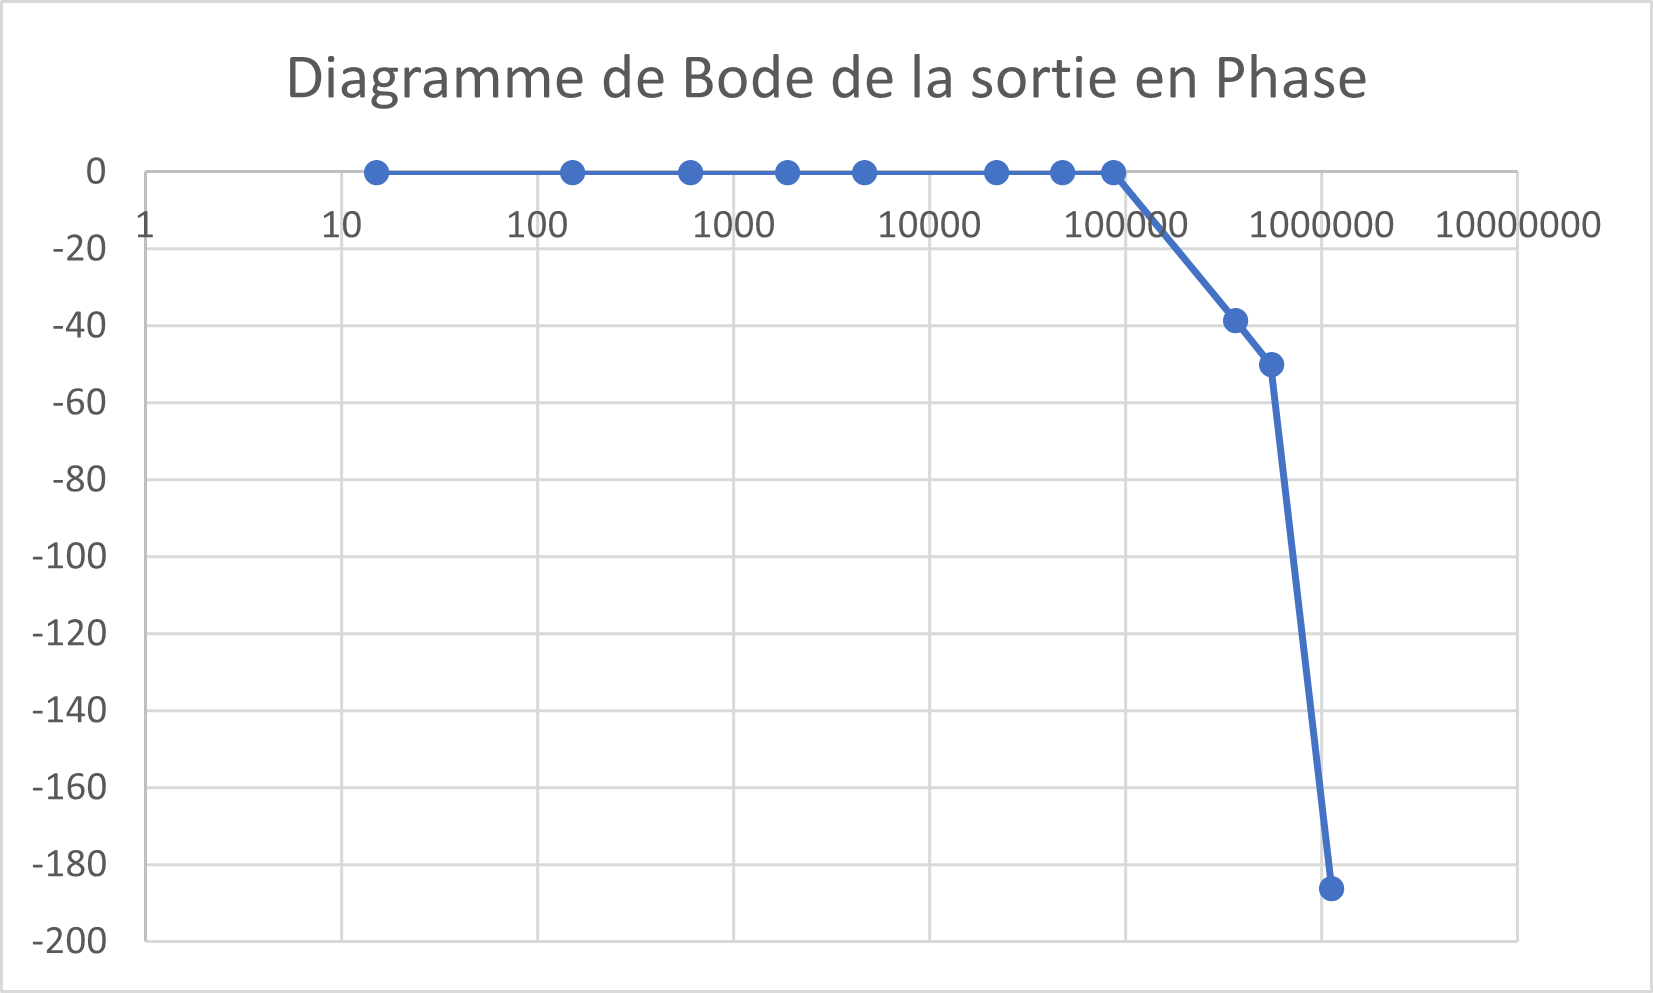
\includegraphics[scale=0.7]{IMAGES/phi_out.png} 
\end{center}
\caption{Diagramme de Bode en phase des sorties}
\label{fig:phiout}
\end{figure}

\thispagestyle{empty}
\printbibliography
\thispagestyle{empty}

\end{document}
